\documentclass[a4paper,12pt]{jarticle}
\usepackage[dvipdfmx]{graphicx}
\usepackage[dvipdfmx]{color}
\usepackage{tabularx}
\topmargin=10mm

\title{物理学実験2 課題6 X線回折}
\author{B6SB2006  石川祐也}
\date{2018/5/22}

\begin{document}

\section{背景と目的}
 原子構造を決定する事は物性を理解する根本的なプロセスである。本課題では、X線回折による結晶構造の
 決定の仕組みを体験するとともに、逆格子の概念やフーリエ変換を理解することを目的とする。

\section{実験原理}
 \subsection{ブラッグの公式}
  ブラッグの公式はnを自然数としたとき、以下の式で与えられる。
  $$2d \sin \theta = n \lambda$$
  これはX線の波に対して原子配列は回折結晶の役割を果たし、各原子からの散乱波が強め合う条件を表している。
  強度の強い反射はn=1の時だけである。
  

 \subsection{距離dと面指数の関係}
  結晶面の面指数が(hkl)であり、格子定数がaであるとき、面間隔dは以下の式で与えられる。
  $$d = \frac{a}{\sqrt{h^2 + k^2 + l^2}}$$

 \subsection{フーリエ変換}
  電子密度マップを求めるためのフーリエ変換の公式は以下の式で与えられる。
  $$\rho(\vec{r})=\frac{1}{(2 \pi)^3}\int d\vec{q} F{\vec{q}} \exp(-i\vec{q}・\vec{r})$$
  ここで逆格子の概念を導入すると、以下のように書き換えることができる。
  $$\rho(\vec{r})=\sum F(hkl) \exp{(-2\pi i(hx+ky+lz))}$$
  今回の実験において使用したコードは巻末に記載する。
  

\section{実験方法}
 \subsection{実験試料}

  \begin{enumerate}
   \item NaCl粉末
   \item KCl粉末
   \item Al粉末
  \end{enumerate}

  \subsection{実験装置}
   \begin{itemize}
    \item 乳鉢・乳棒
    \item 試料ホルダー
    \item X線発生装置
    \item イメージングプレート(IP)
    \item 粉末回折ホルダー
    \item ビームキャプチャー
    \item コリメータ
    \item X線管球部
   \end{itemize}

   \subsection{解析ソフトウェア}
    \begin{itemize}
     \item TRY-IP-READER
     \item TRY-VIEWER
     \item Python 3.6.1
    \end{itemize}

  \subsection{実験手順}

  \renewcommand{\labelenumi}
   {(\arabic{enumi})}

  \begin{enumerate}
   \item 実験試料を丹念にすり潰し、試料ホルダーを作成した。
   \item X線回折装置を用いてIPにX線強度を記録した。
   \item TRY-IP-READERを用いてIPを読み取った。
   \item TRY-VIEWERを用いてデータを書き出した。
   \item Pythonを用いて結晶構造を求めた。ソースコードは巻末に記載した。
  \end{enumerate}


\section{実験結果}
  \subsection{実験1 NaCl結晶構造の特定}
   2$\theta$-強度グラフを図\ref{fig:NaCl_plot}、各データの一覧を表\ref{table:NaCl}、
   z=0,z=0.5における電子密度マップを図\ref{fig:NaCl_im}に示した。


   \begin{figure}[htbp]
    \begin{center}
     \includegraphics[clip,width=12.0cm]{NaCL_plot.png}
     \label{fig:NaCl_plot}
     \caption{2$\theta$-強度グラフ}
    \end{center}
   \end{figure}

   \begin{table}[htbp]
    \begin{center}

       \caption{NaClにおける各データの一覧}
        \begin{tabular}{|r|r|r|r|r|r|r|}
         \hline
                 hkl   &     111   &     200   &     220   &       222 &       400 &       420 \\
         \hline
			2$\theta$  & 12.584072 & 14.540293 & 20.630895 & 25.354746 & 29.373919 & 32.965019 \\
			distance   & 3.250482  & 2.815000  & 1.990506  & 1.625241  & 1.407500  & 1.258906 \\
			I(hkl)   & 2.483306  & 646.186757 & 164.468498 &  9.917789 &  1.469235 &  6.885137 \\
         \hline

         \hline
        \end{tabular}
       \label{table:NaCl}

      \end{center}
     \end{table}
     
     \begin{figure}[htbp]
      \begin{center}
       \begin{tabular}{c}
       
       %1
       \begin{minipage}{0.5\hsize}
        \begin{center}
         \includegraphics[clip,width=8cm]{NaCL_im00.png}
         \label{fig:NaCl_im00}
         \hspace{1.6cm} [1]z=0
        \end{center}
       \end{minipage}
       
       %2
       \begin{minipage}{0.5\hsize}
        \begin{center}
         \includegraphics[clip,width=8cm]{NaCL_im05.png}
         \label{fig:NaCl_im05}
         \hspace{1.6cm} [2]z=0.5
        \end{center}
       \end{minipage}
       
      \end{tabular} 
      \caption{電子密度マップ}
      \label{fig:NaCl_im}
      \end{center}
     \end{figure}  
        
  \subsection{実験2 KCl結晶構造の特定}
   2$\theta$-強度グラフを図\ref{fig:KCl_plot}、各データの一覧を表\ref{table:KCl}、
   z=0,z=0.5における電子密度マップを図\ref{fig:KCl_im}に示した。


   \begin{figure}[htbp]
    \begin{center}
     \includegraphics[clip,width=12.0cm]{KCL_plot.png}
     \label{fig:KCl_plot}
     \caption{2$\theta$-強度グラフ}
    \end{center}
   \end{figure}

   \begin{table}[htbp]
    \begin{center}

       \caption{KClにおける各データの一覧}
        \begin{tabular}{|r|r|r|r|r|r|r|}
         \hline
                 hkl   &     200   &     220   &       222 &       400 &       420 &      422 \\
         \hline
			2$\theta$  & 12.848988 & 18.314135 & 22.483611 & 26.070175 & 29.320779 & 32.312745 \\
			distance   &  3.140000 &  2.220315 &  1.812880 &  1.570000 &  1.404251 &  1.281900\\
			I(hkl)   &  211.822263 & 60.561554 &  7.789260 &  0.297566 &  3.369641 &  1.135681\\
         \hline

         \hline
        \end{tabular}
       \label{table:KCl}

      \end{center}
     \end{table}
     
     \begin{figure}[htbp]
      \begin{center}
       \begin{tabular}{c}
       
       %1
       \begin{minipage}{0.5\hsize}
        \begin{center}
         \includegraphics[clip,width=8cm]{KCL_im00.png}
         \label{fig:KCl_im00}
         \hspace{1.6cm} [1]z=0
        \end{center}
       \end{minipage}
       
       %2
       \begin{minipage}{0.5\hsize}
        \begin{center}
         \includegraphics[clip,width=8cm]{KCL_im05.png}
         \label{fig:KCl_im05}
         \hspace{1.6cm} [2]z=0.5
        \end{center}
       \end{minipage}
       
      \end{tabular} 
      \caption{電子密度マップ}
      \label{fig:KCl_im}
      \end{center}
     \end{figure}  

   
  \subsection{実験3 Al結晶構造の特定}
   2$\theta$-強度グラフを図\ref{fig:Al_plot}、各データの一覧を表\ref{table:Al}、
   z=0,z=0.5における電子密度マップを図\ref{fig:Al_im}に示した。


   \begin{figure}[htbp]
    \begin{center}
     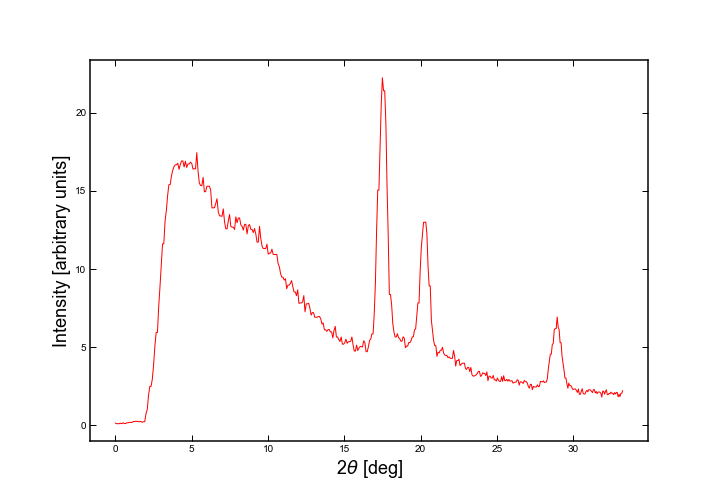
\includegraphics[clip,width=12.0cm]{Al_plot.png}
     \label{fig:Al_plot}
     \caption{2$\theta$-強度グラフ}
    \end{center}
   \end{figure}

   \begin{table}[htbp]
    \begin{center}

       \caption{Alにおける各データの一覧}
        \begin{tabular}{|r|r|r|r|r|r|r|}
         \hline
                 hkl   &     111   &     200   &     220   \\
         \hline
			2$\theta$  & 17.518690 & 20.242201 & 28.896402 \\
			distance   &  2.338269 &  2.025000 & 1.4318913 \\
			I(hkl)     & 119.543988 & 41.426174 & 10.754482 \\
         \hline

         \hline
        \end{tabular}
       \label{table:Al}

      \end{center}
     \end{table}
     
     \begin{figure}[htbp]
      \begin{center}
       \begin{tabular}{c}
       
       %1
       \begin{minipage}{0.5\hsize}
        \begin{center}
         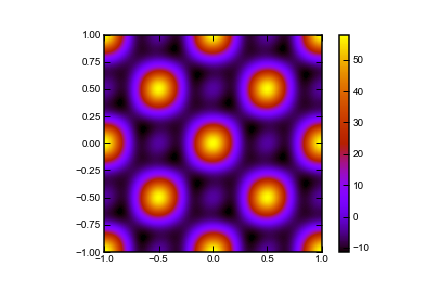
\includegraphics[clip,width=8cm]{Al_im00.png}
         \label{fig:Al_im00}
         \hspace{1.6cm} [1]z=0
        \end{center}
       \end{minipage}
       
       %2
       \begin{minipage}{0.5\hsize}
        \begin{center}
         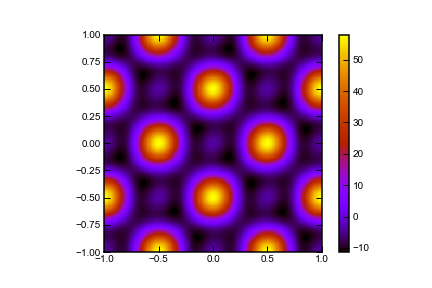
\includegraphics[clip,width=8cm]{Al_im05.png}
         \label{fig:Al_im05}
         \hspace{1.6cm} [2]z=0.5
        \end{center}
       \end{minipage}
       
      \end{tabular} 
      \caption{電子密度マップ}
      \label{fig:Al_im}
      \end{center}
     \end{figure}  
     
\section{結果の考察}
 NaClの電子密度マップは、原子1つ毎に濃淡がある様子が見て取れる。またその濃淡がz=0とz=0.5では
 入れ替わることが分かる。イオンにおける電子数を考えると、電子密度マップで濃い原子は塩素であり、
 電子密度マップで淡い原子はナトリウムであると考えられる。以上のことからNaCl結晶が面心立方の結晶構造を
 持つ事が確かめられた。\\
  一方、KClの電子密度マップは、原子1つ毎の濃淡が見て取れない。これはカリウムイオン及び塩化物イオンがアルゴンの電子配置
 を取るため、X線では見分ける事ができないためであると考えられる。KCl結晶の原子を見分けるためには、陽子数が違うことから
 中性子線での散乱を測定すべきであると考えられる。\\
  Alにおいてはz=0とz=0.5において原子の配列が入れ替わることが分かる。このことからAl結晶が面心立方の結晶構造を
 持つ事が確かめられた。
  

\section{結論}
 各結晶においてフーリエ変換を用いて電子密度マップを求めることが出来た。これらを通して結晶構造の決定の仕組みについて
 理解する事が出来た。またコンピュータを用いたフィッティングの技術を習得することが出来た。

\section{マニュアルの問題}
 (a)~(d)においては、結果の項に記載したのでそちらに代える。
 (e)においては別紙1に記載した。
 
\section{教科書の問題}
 演習問題は別紙2に記載した。
 
\section{appendix}
 【ソースコード】
  \begin{figure}[htbp]
    \begin{center}
     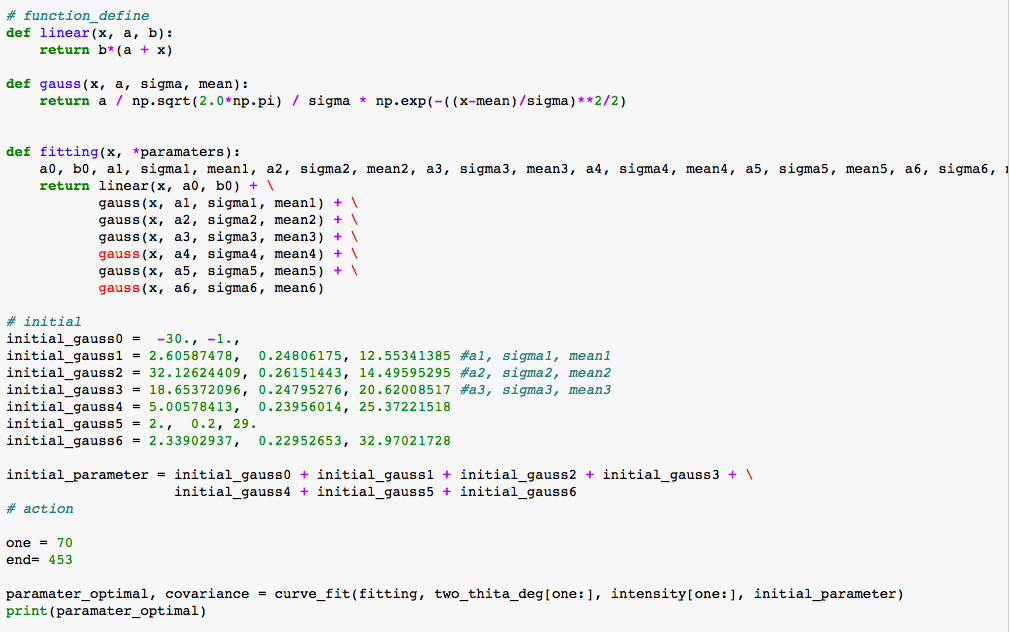
\includegraphics[clip,width=14.0cm]{py_1.png}
     
    \end{center}
  \end{figure}
  
  \begin{figure}[htbp]
    \begin{center}
     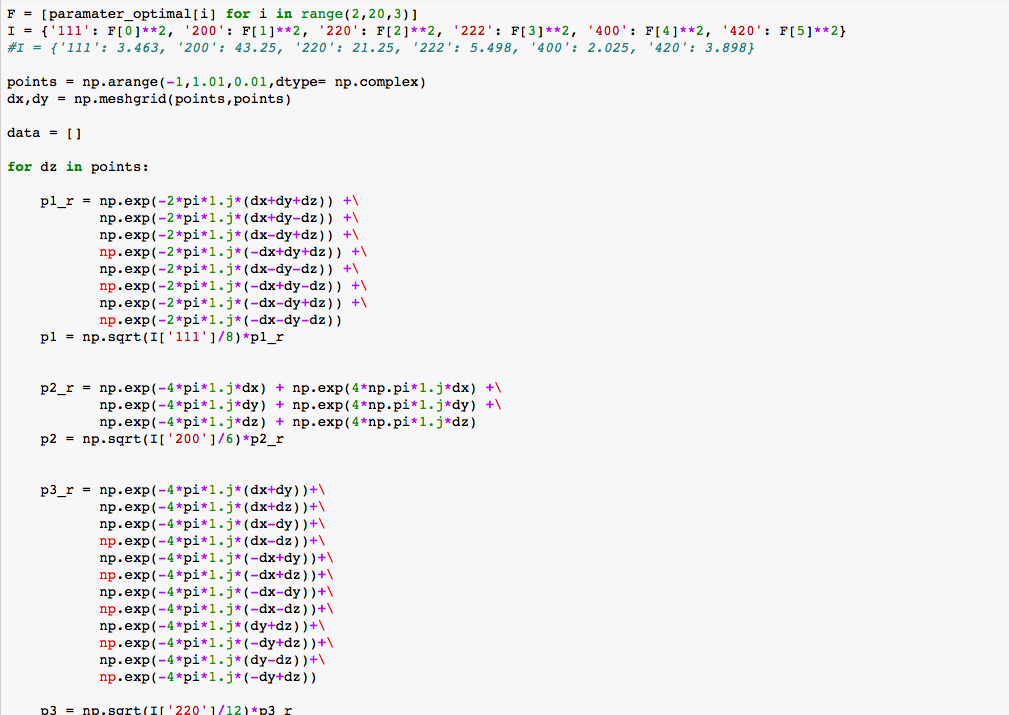
\includegraphics[clip,width=14.0cm]{py_2.png}
     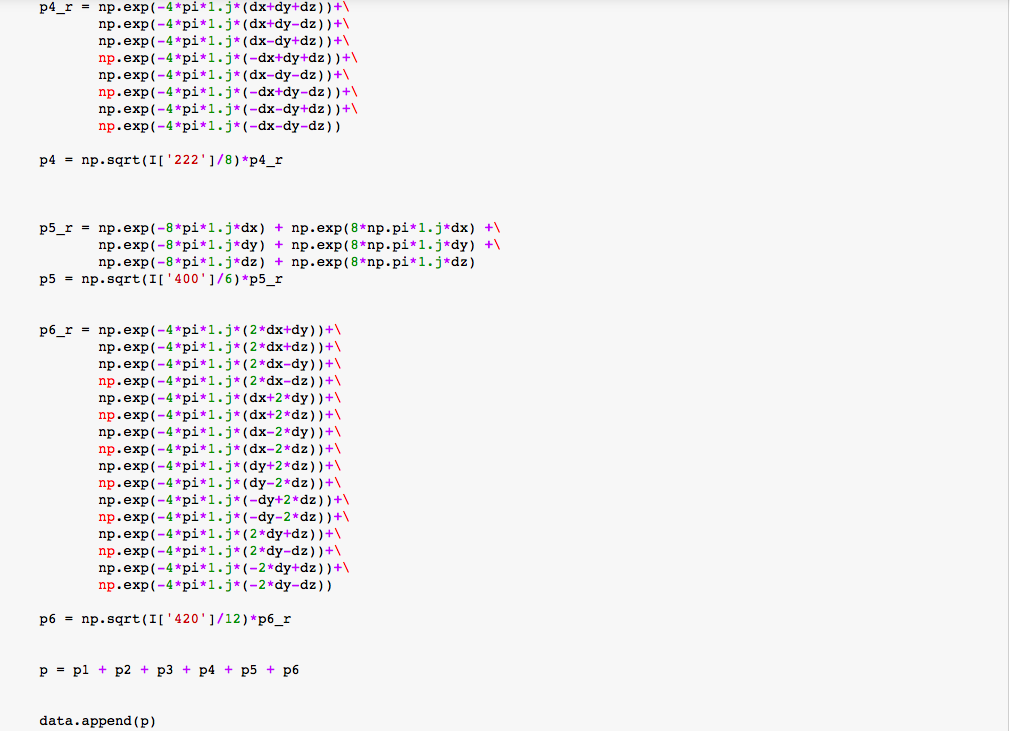
\includegraphics[clip,width=14.0cm]{py_3.png}
     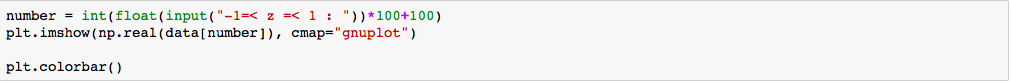
\includegraphics[clip,width=14.0cm]{py_4.png}
    \end{center}
   \end{figure}
  

\end{document}
